\documentclass[11pt,a4paper]{article}
\usepackage[utf8]{inputenc}
\usepackage[T1]{fontenc}
\usepackage{amsmath,amssymb}
\usepackage{geometry}
\geometry{margin=2.5cm}
\usepackage{booktabs}
\usepackage{array}
\usepackage{xcolor}
\usepackage{tikz}
\usepackage{tcolorbox}
\tcbuselibrary{skins,breakable}

% Colori
\definecolor{nodecolor}{RGB}{30,100,200}
\definecolor{edgecolor}{RGB}{200,80,30}
\definecolor{clusterA}{RGB}{52,152,219}
\definecolor{clusterB}{RGB}{231,76,60}
\definecolor{boxbg}{RGB}{245,248,255}

\newtcolorbox{stepbox}[2][]{
  colback=boxbg, colframe=nodecolor!60!black,
  fonttitle=\bfseries, title={#2}, #1,
  left=6pt, right=6pt, top=4pt, bottom=4pt
}

\title{\textbf{Esempio Numerico --- GNN per Antenna Clustering}\\[4pt]
\large Griglia $2\times2$, $K=2$ cluster, dimensioni ridotte}
\author{}
\date{}

\begin{document}
\maketitle

% ============================================================
\section*{Setup: griglia $2\times2$}
% ============================================================

\begin{center}
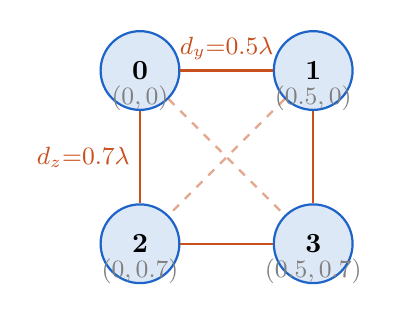
\begin{tikzpicture}[node distance=2.2cm,
  ant/.style={circle, draw=nodecolor, fill=nodecolor!15, thick,
              minimum size=1cm, font=\bfseries}]
  \node[ant] (0) at (0,0)   {0};
  \node[ant] (1) at (2.2,0) {1};
  \node[ant] (2) at (0,-2.2){2};
  \node[ant] (3) at (2.2,-2.2){3};
  % 4-connected
  \draw[thick,edgecolor] (0)--(1) node[midway,above,font=\small]{$d_y{=}0.5\lambda$};
  \draw[thick,edgecolor] (0)--(2) node[midway,left, font=\small]{$d_z{=}0.7\lambda$};
  \draw[thick,edgecolor] (1)--(3);
  \draw[thick,edgecolor] (2)--(3);
  % diagonali (8-connected)
  \draw[thick,edgecolor,dashed,opacity=0.5] (0)--(3);
  \draw[thick,edgecolor,dashed,opacity=0.5] (1)--(2);
  % label posizioni
  \node[below=2pt,font=\small\color{gray}] at (0) {$(0,0)$};
  \node[below=2pt,font=\small\color{gray}] at (1) {$(0.5,0)$};
  \node[below=2pt,font=\small\color{gray}] at (2) {$(0,0.7)$};
  \node[below=2pt,font=\small\color{gray}] at (3) {$(0.5,0.7)$};
\end{tikzpicture}
\end{center}

\medskip
\noindent
4 antenne, archi continui = 4-connected, archi tratteggiati = diagonali (8-connected).
Parametri toy: \texttt{hidden\_dim}$=2$, $K=2$, 1 attention head, $W_{\text{proj}}=I$.

\begin{center}
\renewcommand{\arraystretch}{1.3}
\begin{tabular}{ccc}
\toprule
\textbf{Nodo} & \textbf{Posizione} $(y,z)$ in $\lambda$ & \textbf{Feature vettore} $\mathbf{x}_i$\\
\midrule
0 & $(0.0,\ 0.0)$ & $[0.0,\ 0.0]$\\
1 & $(0.5,\ 0.0)$ & $[0.5,\ 0.0]$\\
2 & $(0.0,\ 0.7)$ & $[0.0,\ 0.7]$\\
3 & $(0.5,\ 0.7)$ & $[0.5,\ 0.7]$\\
\bottomrule
\end{tabular}
\end{center}

% ============================================================
\section*{Step 1 --- Input Projection}
% ============================================================

\begin{stepbox}{Input Projection: Linear $(2\!\to\!2)$ + BatchNorm + ELU}
Con $W_{\text{proj}} = I$ e normalizzazione trascurabile sui valori toy:

\[
H^{(0)} = \begin{pmatrix}0 & 0\\0.5 & 0\\0 & 0.7\\0.5 & 0.7\end{pmatrix}
\quad\in\mathbb{R}^{4\times 2}
\]

Ogni riga = embedding iniziale del nodo, che a questo punto coincide con la posizione fisica.
\end{stepbox}

% ============================================================
\section*{Step 2 --- GAT: Attention Score su un arco}
% ============================================================

\begin{stepbox}{Attention score $e_{01}$ per l'arco nodo~0~$\to$~nodo~1}
Le \textbf{edge features} dell'arco $(0\to1)$ sono:
\[
\mathbf{e}_{01} = [\Delta y,\ \Delta z,\ \text{dist}] = [0.5,\ 0.0,\ 0.5]
\]

Il GAT concatena embedding sorgente, destinazione ed edge features e applica un vettore di attenzione $\mathbf{a}$:
\[
e_{01} = \text{LeakyReLU}\!\left(\mathbf{a}^\top
\bigl[\underbrace{W\mathbf{h}_0}_{\text{sorgente}}\;\|\;\underbrace{W\mathbf{h}_1}_{\text{dest}}\;\|\;\underbrace{\mathbf{e}_{01}}_{\text{edge}}\bigr]\right)
\]

Con $W=I$ e $\mathbf{a}=\mathbf{1}$:
\[
e_{01} = \text{LReLU}\!\underbrace{(0+0)}_{\mathbf{h}_0}
         \underbrace{{}+0.5+0}_{\mathbf{h}_1}
         \underbrace{{}+0.5+0+0.5}_{\mathbf{e}_{01}}
       = \text{LReLU}(1.5) = 1.5
\]

\medskip
Ripetiamo per tutti i vicini del nodo~0 (8-connected: nodi 1, 2, 3):

\begin{center}
\begin{tabular}{cccc}
\toprule
Vicino $j$ & $\mathbf{h}_j$ & Edge dist & $e_{0j}$\\
\midrule
1 & $[0.5, 0.0]$ & $0.5\lambda$ & $1.5$\\
2 & $[0.0, 0.7]$ & $0.7\lambda$ & $1.4$\\
3 & $[0.5, 0.7]$ & $0.86\lambda$ (diag.) & $2.2$\\
\bottomrule
\end{tabular}
\end{center}

\medskip
\textbf{Softmax} sui raw scores $\to$ coefficienti di attenzione $\alpha_{0j}$:
\[
\alpha_{0j} = \frac{\exp(e_{0j})}{\sum_{k\in\mathcal{N}(0)}\exp(e_{0k})}
\]
\[
\alpha_{01} = \frac{e^{1.5}}{e^{1.5}+e^{1.4}+e^{2.2}}
            = \frac{4.48}{4.48+4.06+9.03} = 0.26
\]
\[
\alpha_{02} = 0.23,\qquad \alpha_{03} = 0.51
\]

Il nodo~3 (diagonale con embedding più ricco) pesa di più. Ha senso: è il nodo più ``informativo'' per capire in quale cluster collocare il nodo~0.
\end{stepbox}

% ============================================================
\section*{Step 3 --- GAT: Aggregazione per il nodo~0}
% ============================================================

\begin{stepbox}{Nuovo embedding $\mathbf{h}_0^{(1)}$ dopo un layer GAT}
\[
\mathbf{h}_0^{(1)} = \text{ELU}\!\left(\sum_{j\in\mathcal{N}(0)}\alpha_{0j}\cdot W\mathbf{h}_j\right)
\]
\[
= \text{ELU}\!\left(
  0.26\begin{pmatrix}0.5\\0\end{pmatrix}
+ 0.23\begin{pmatrix}0\\0.7\end{pmatrix}
+ 0.51\begin{pmatrix}0.5\\0.7\end{pmatrix}
\right)
\]
\[
= \text{ELU}\!\left(\begin{pmatrix}0.13+0+0.255\\0+0.161+0.357\end{pmatrix}\right)
= \text{ELU}\!\left(\begin{pmatrix}0.385\\0.518\end{pmatrix}\right)
\approx \begin{pmatrix}0.385\\0.518\end{pmatrix}
\]

\textbf{Interpretazione}: il nodo~0 ha ``guardato'' i suoi vicini pesati per accoppiamento e distanza. Il suo nuovo embedding codifica non solo la sua posizione, ma anche il contesto spaziale del suo vicinato.
\end{stepbox}

% ============================================================
\section*{Step 4 --- Gumbel-Softmax e Assegnazione ai Cluster}
% ============================================================

\begin{stepbox}{Classifier + Gumbel-Softmax ($\tau = 0.5$)}
Dopo 3 layer GAT, il classificatore lineare produce i \textbf{logits} per $K=2$:

\[
\text{logits}_i = W_{\text{clf}}\,\mathbf{h}_i^{(3)}
\]

\begin{center}
\begin{tabular}{ccc}
\toprule
Nodo & $\text{logit}_{\text{cluster 0}}$ & $\text{logit}_{\text{cluster 1}}$\\
\midrule
0 & $+1.2$ & $-0.4$\\
1 & $+1.0$ & $-0.3$\\
2 & $-0.6$ & $+1.3$\\
3 & $-0.5$ & $+1.1$\\
\bottomrule
\end{tabular}
\end{center}

\medskip
Durante il \textbf{training}, si campiona il rumore Gumbel $g_i \sim -\log(-\log U_i)$, $U_i\sim\mathcal{U}(0,1)$:
\[
g = (-0.3,\ 0.8)\quad\text{(esempio campionato per il nodo~0)}
\]

Si applica la \textbf{Gumbel-Softmax}:
\[
z_{0,k} = \frac{\exp\!\bigl((\text{logit}_{0,k}+g_k)/\tau\bigr)}{\sum_{j}\exp\!\bigl((\text{logit}_{0,j}+g_j)/\tau\bigr)}
= \frac{\exp\!\bigl((0.9,\ 0.4)/0.5\bigr)}{Z}
= \text{softmax}(1.8,\ 0.8)
\]
\[
z_0 = \left(\frac{e^{1.8}}{e^{1.8}+e^{0.8}},\ \frac{e^{0.8}}{e^{1.8}+e^{0.8}}\right) = (0.73,\ 0.27)
\]

Senza rumore Gumbel (eval), si usa il softmax standard diviso per $\tau$.
\end{stepbox}

% ============================================================
\section*{Risultato: Matrice di Assegnazione $Z$}
% ============================================================

\[
Z = \begin{pmatrix}
0.73 & 0.27\\
0.68 & 0.32\\
0.29 & 0.71\\
0.31 & 0.69
\end{pmatrix}
\in\mathbb{R}^{4\times 2}
\]

\begin{center}
\renewcommand{\arraystretch}{1.4}
\begin{tabular}{cccc}
\toprule
\textbf{Nodo} & $z_{i,0}$ (prob cluster 0) & $z_{i,1}$ (prob cluster 1) & \textbf{Assegnazione hard}\\
\midrule
0 & $0.73$ & $0.27$ & \textcolor{clusterA}{\textbf{Cluster 0}}\\
1 & $0.68$ & $0.32$ & \textcolor{clusterA}{\textbf{Cluster 0}}\\
2 & $0.29$ & $0.71$ & \textcolor{clusterB}{\textbf{Cluster 1}}\\
3 & $0.31$ & $0.69$ & \textcolor{clusterB}{\textbf{Cluster 1}}\\
\bottomrule
\end{tabular}
\end{center}

\medskip
\begin{center}
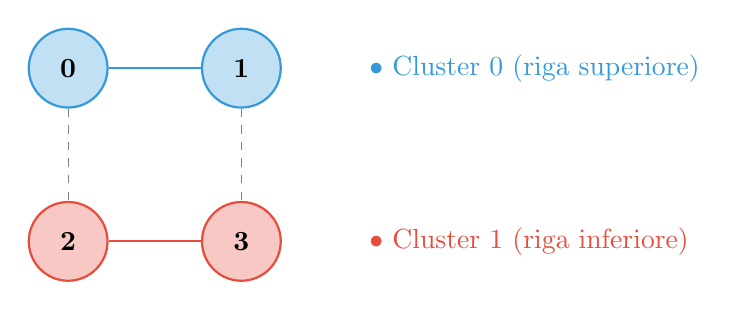
\begin{tikzpicture}[
  ant/.style={circle, draw, thick, minimum size=1cm, font=\bfseries}]
  \node[ant, fill=clusterA!30, draw=clusterA] (0) at (0,0)    {0};
  \node[ant, fill=clusterA!30, draw=clusterA] (1) at (2.2,0)  {1};
  \node[ant, fill=clusterB!30, draw=clusterB] (2) at (0,-2.2) {2};
  \node[ant, fill=clusterB!30, draw=clusterB] (3) at (2.2,-2.2){3};
  \draw[thick,clusterA] (0)--(1);
  \draw[thick,clusterB] (2)--(3);
  \draw[gray,dashed] (0)--(2);
  \draw[gray,dashed] (1)--(3);
  \node[right=1.5cm] at (1) {\textcolor{clusterA}{$\bullet$ Cluster 0 (riga superiore)}};
  \node[right=1.5cm] at (3) {\textcolor{clusterB}{$\bullet$ Cluster 1 (riga inferiore)}};
\end{tikzpicture}
\end{center}

La riga superiore finisce in un cluster, quella inferiore nell'altro: fisicamente contigui, risultato sensato.

% ============================================================
\section*{Perché Gumbel-Softmax e non Softmax diretto?}
% ============================================================

\begin{center}
\renewcommand{\arraystretch}{1.4}
\begin{tabular}{p{3.5cm} p{5cm} p{5cm}}
\toprule
& \textbf{Softmax standard} & \textbf{Gumbel-Softmax}\\
\midrule
Output & Distribuzione di probabilità morbida & Campione differenziabile quasi-discreto\\
Gradienti & Fluiscono sempre & Fluiscono (approximation)\\
Discretezza & Nessuna ($z$ sempre continuo) & Controllata dal parametro $\tau$\\
Training & Stabile ma cluster sfumati & Cluster più netti a $\tau$ basso\\
\midrule
\multicolumn{3}{l}{\textbf{Regola pratica}: inizia con $\tau=1.0$ e anneal verso $\tau\approx0.2$ durante il training.}\\
\bottomrule
\end{tabular}
\end{center}

\[
\tau\to 0: \quad z_i \to \text{one-hot} \quad\text{(discreto, gradienti instabili)}
\]
\[
\tau\to\infty: \quad z_i \to \text{uniforme} \quad\text{(molto morbido, poca info)}
\]

\end{document}
